\chapter{Udviklingen}\label{ch:Udviklingen}
%%Husk at få kilder på alle vigtige ord / udtryk fra Scrum, XP og kanban (fx Product Owner, sprint backlog, scrum master, etc.)
Nedstående sektioner vil sætte brugen af agile metoder i fokus, samt hvordan udviklingen af systemet er foregået.

\section{Brug af Scrum}

Scrum har været en central del af hvordan dette projekt er blevet udviklet.
For at danne et bedre overblik over hvordan gruppen har benyttet Scrum, vil de 9 forskellige Scrum roller, ceremonier(+2) og artifakter blive gennemgået. Afsnittet vil primært indeholde de dele som er benyttet i den nævnte rækkefølge.

\subsection{Roller}

En af de centrale roller i Scrum er Product Owner. 
%Product Owner er den som står til ansvar for succes eller fiasko af projektet, bestemmer retningen af projektet og har fokus på at projektet skal skabe mest mulig værdi for brugerne af systemet. Det er også Product Owner som har til ansvar at håndtere product backlog og sørge for at den er opdateret og relevant.
Product Owner i dette projekt har været teamet selv, netop fordi det er et lille team, som er uerfaren med hvordan et Scrum projekt skal fungere. Siden teamet har valgt at håndtere rollen som Product Owner, betyder dette at alle har haft en indflydelse på hvilke features, der skulle være centrale i projektet. Det samme gælder prioritering af user stories i product backloggen, samt andre tekniske funktioner af produktet. 

%Scrum Master har til opgave at sørge for mål, scope, og produktdomænet er indforstået blandt alle gruppemedlemmer. Dette betyder at det også er Scrum Master der har ansvar for at oprette Scrum møder, og hjælpe Development Teamet til at gennemføre deres opgaver. 
Vedrørende Scrum Master er det samme princip ikke brugt, som Product Owner. Hvad der menes med dette, er at Scrum Master denne gang har været én person, dog med en rolle-rokering for hvert sprint. 
%I feel like we're not talking about how good/bad this worked, and more about what the Scrum Master ended up doing this project.

Nu da de 2 første roller er gennemgået, er det denne gang udviklingsteamet, som skal tages i overvejelse. Med en gruppe på blot 4 personer har beslutningen for denne rolle været, at hele teamet er en del af udviklingsteamet. Det menes, at denne beslutning vil skabe den bedste værdi for hver enkelt individ, så alle har et overblik over hvordan arkitekturen er, og at alle er med til at udvikle systemet hele vejen fra story til færdig implementeret feature.

Som forklaret har alle gruppemedlemmer flere roller samtidig i dette projekt, hvilket kan skabe noget forvirring om, hvordan man skal agere ift. andre i projektet. Beslutningen om at påtage sig flere roller ad gangen er som nævnt taget på baggrund af, at alle i gruppen kan sætte sig ind i rollerne. Desuden virker det unødvendigt at have inaktive Product Owner og Scrum Master når der skal udvikles videre på projektet - især da der ikke er andre administrative og kunderelaterede opgaver de skal tage sig af dette projekt.



\subsection{Ceremonier}

Teamet startede projektet ud med Sprint Planning\cite{ScrumTrenches}, hvor der blev dannet 8 forskellige user stories, som blev benyttet til at danne en product backlog.Sammen blev der diskuteret prioritering, og tilføjet ID og korte beskrivelser af ønskede funktioner til produktet. Ud fra denne product backlog har teamet  kunne oprette en sprint backlog, på baggrund af hvad der er prioriteret højst på product backloggen. Herfra har teamet oprettet en liste over alle opgaver der skal udføres, med et estimat af tidsfordeling på opgaver ved hjælp af planning poker\cite{ScrumTrenches}. Sprint backloggen er blevet opdateret hver eneste dag. Nederest er det muligt at se 3 forskellige eksempler, der viser teamets egen product backlog, sprint backlog og det burndown chart teamet har oprettet for at illustrere hvor langt man er i forhold til planen. 

\subsection{Artifakter}

I sprint 0 sørgede teamet for at danne et godt overblik, over hvilke opgaver der havde den højste prioritet. Det valgte egenskaber blev så tilføjet til sprint backloggen, selvfølgelig henblik på hvor stor en opgave det er, så teamet ikke blev overvældet af mængden af opgaver. Efter denne proces, var det tid til at estimerer opgaverne. Dette blev gjort i brug af planning poker. Når så alle opgaverne var estimeret og fordelt til forskellige team medlemmer, blev projektet sat i gang. Herfra har teamet ydet for at opnå såvidt som det nu kunne lade sig gøre, at følge ceremonierne. De daglige Scrum møder, har ikke altid været daglige, på grund af undervisning eller forglemmelse af at informerer teamet, om mødetidspunkt, men teamet har til gengæld været gode til at opdaterer på processen overfor hindanden. For hvert nyt sprint, har denne proces gentaget sig, med opdateringer på product backlog og en reflektion / evaluering af sprintet. 



\section{Brug af XP med Scrum}

Som tidligere nævnt har teamet benyttet Scrum som den centrale udviklingsmetode, dog er der også XP elementer, som teamet har implementeret i processen. Herunder Pair Programming, Small Releases, Test Driven Develoment (TDD), Collective Ownership, Continuous Integration, Sustainable Pace og Coding Standards. Så når teamet eksempelvis skal planlægge et sprint, er der benyttet Planning Poker som kommer fra XP. 

Ved hver planlægning af næste sprint brugte vi Planning Poker til at finde ud af hvor mange timer, der skulle afsættes til hver opgave. Dette fungerede godt, og var ovenikøbet en sjov oplevelse, som gjorde det nemmere at estimaterne. I pre-sprint og sprint 0 glemte vi at opveje disse estimater mod vores kapacitet for sprintet, hvilket betød vi endte med at have for mange forventede arbejdstimer ift. hvor mange timer der var tilgængeligt at arbejde i. Til gengæld fik vi stadig nået meget og fik det også dokumenteret til senere. 

Til udviklingen brugte vi TDD for at sikre at de features, der skulle implementeres virkede før det integration. Der er blevet lavet unit- og integrationstest, og front-end har også været igennem flere iterationer for at opnå den bedste brugervenlige navigation. 
Det meste udvikling foregik ved Pair Programming, hvor man sad 2-og-2 om ét tastatur, til at skrive kode. Det har betydet at alle er indforstået med hvad for noget kode der er skrevet, og hvordan det virker, samt hvilken funktion i systemet det har. 
Collective ownership har betydet, at vi alle sammen i gruppen har haft indflydelse på, hvad målet med projektet er, samt hvilken retning det skal styres i. Det har givet godt overblik over hele projektet for samtlige gruppemedlemmer, og har sørget for at der tages beslutninger som alle er enige om.

Alt dette betyder såvidt også, at der kan være risiko for, at projektet ikke vil lykkedes. Derfor er det vigtigt, at analysere og definere risici. Dette er sat i fokus i næste afsnit, som graver mere i dybden med hvordan teamet har håndteret risici der kan være involveret i et projekt som dette.


\begin{figure}
    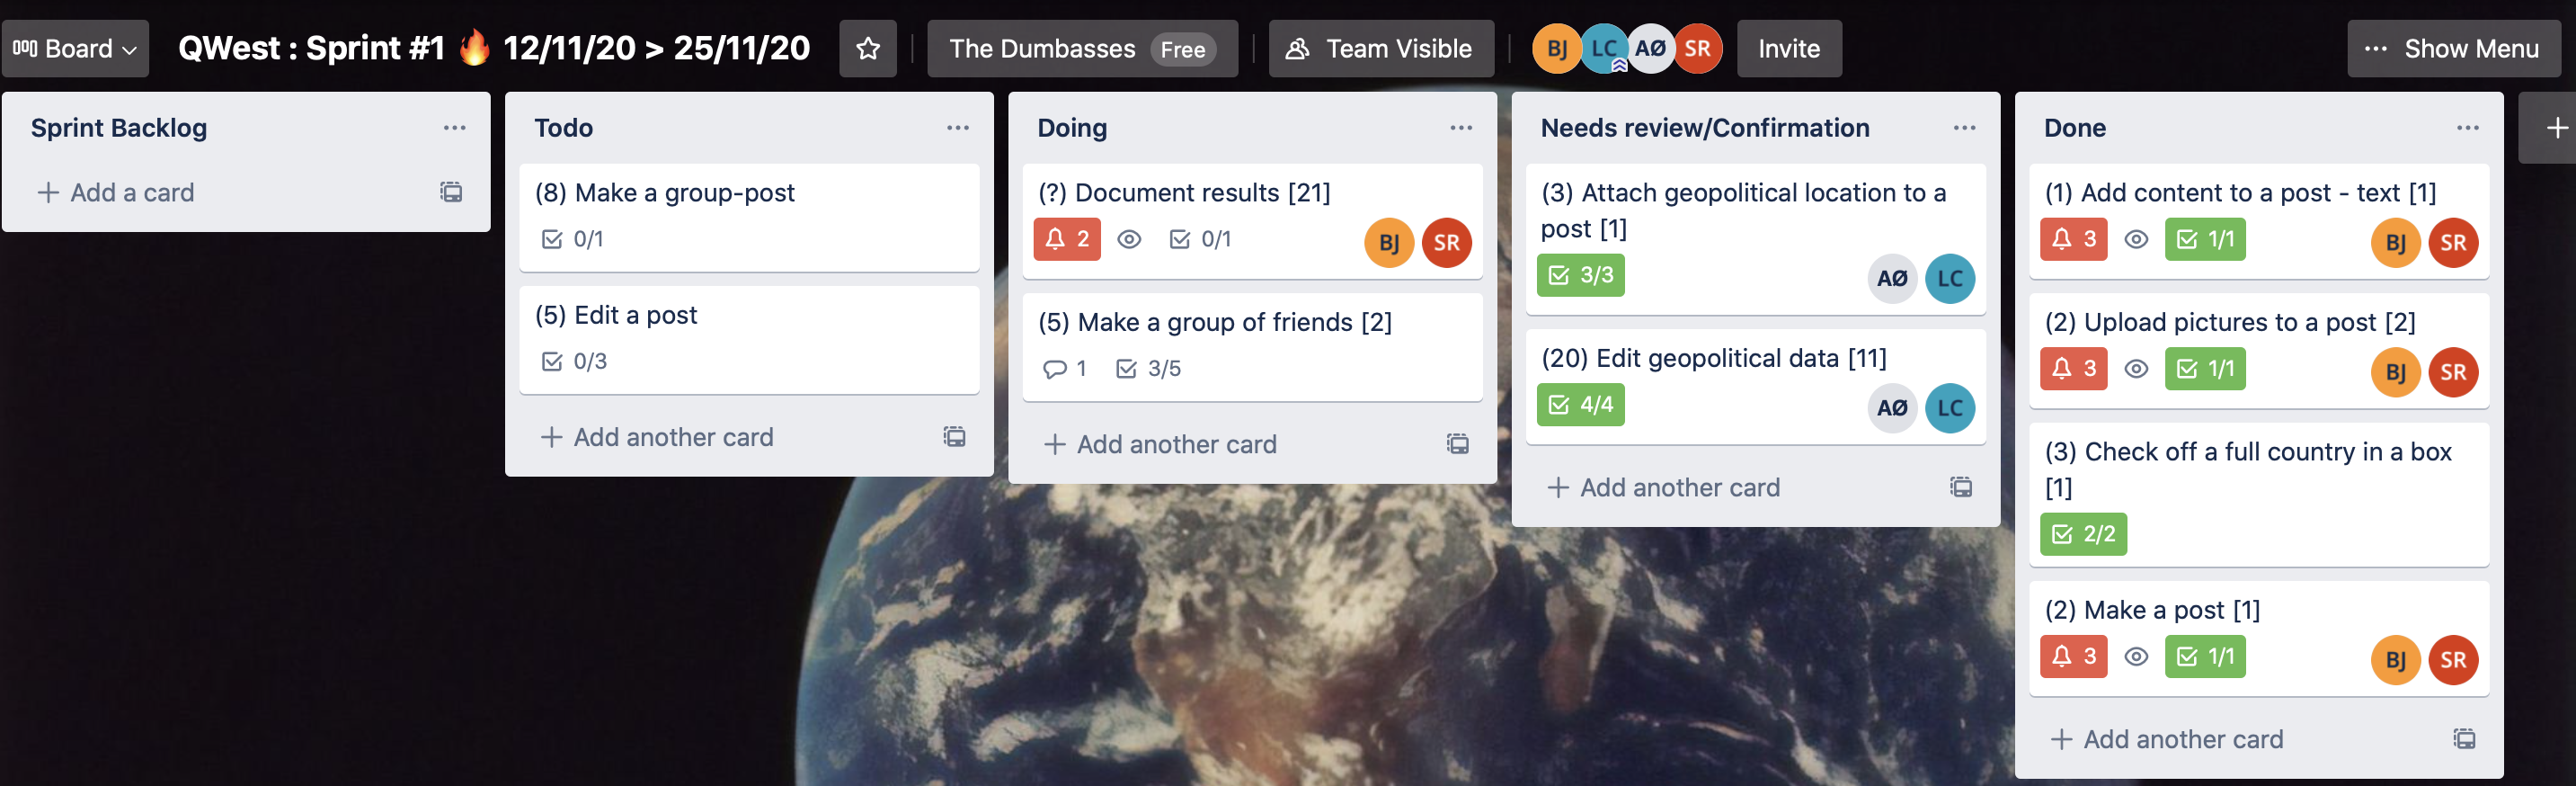
\includegraphics[width=\linewidth]{figures/SprintBacklog.png}
    \caption{Eksempel på et af gruppens Sprint Backlog lavet i Trello}
    \label{fig:Sprint}
\end{figure}


\begin{figure}
    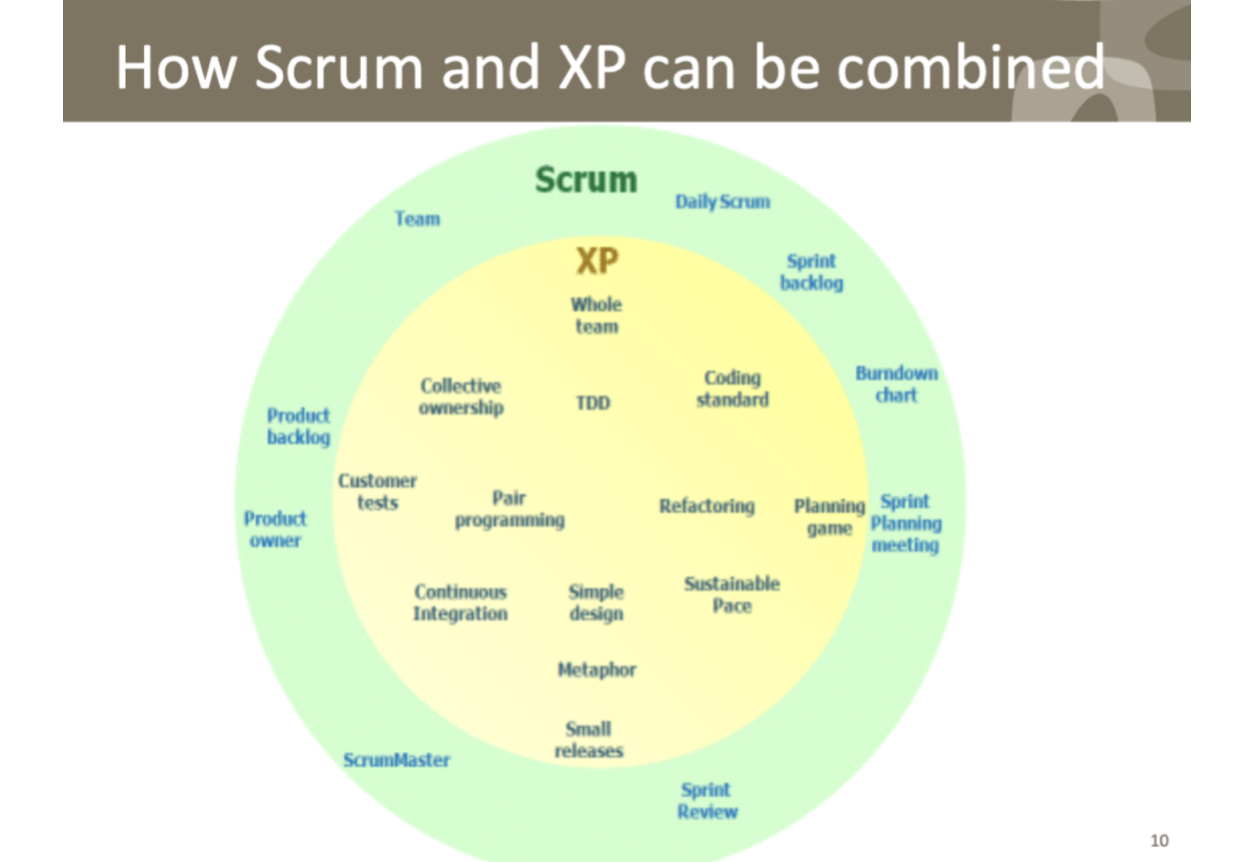
\includegraphics[width=\linewidth]{figures/XP&Scrum.png}
    \caption{Kombinationen af Scrum og XP}
    \label{fig:Kombi}
\end{figure}

